% Cost-accuracy frontier (single-column; compile with -jobname=fig_pareto).
% Carries the accuracy-cost-guarantee boundary: full-contract emulation pays ~115k
% prompt tokens per query for parity (MultiGov), degradation (ICT), or the disclosed
% private win (p=.0039); compilation reproduces its public references at zero online
% calls. Colors: blue=CaliberGraph (stars), neutral gray=frontier emulation arms,
% red dashed box = disclosed private inversion. All text >= 9pt Helvetica; lines >= 0.5pt.
\documentclass[10pt]{standalone}
\usepackage{helvet}
\usepackage{tikz}
\usepackage{pgfplots}
\pgfplotsset{compat=1.17, major tick length=2pt,
  every axis/.append style={axis line style={line width=0.5pt}},
  every tick/.append style={line width=0.5pt, black},
  every mark/.append style={line width=0.5pt}}
\usetikzlibrary{arrows.meta}
\begin{document}
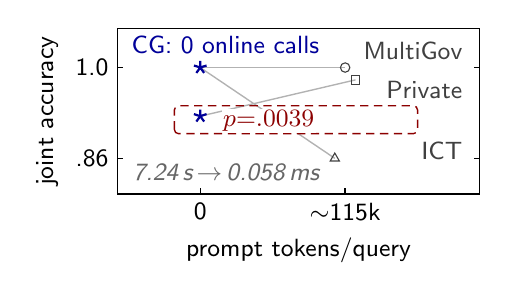
\begin{tikzpicture}
\small\sffamily
\begin{axis}[
  at={(8mm,0mm)}, anchor=south west, scale only axis, width=46mm, height=21mm,
  xmin=0, xmax=3.5, xtick={0.8,2.2}, xticklabels={0,$\sim$115k}, xtick pos=bottom,
  ymin=0.805, ymax=1.06, ytick={.86,1.0}, yticklabels={.86,1.0},
  xlabel={prompt tokens/query}, ylabel={joint accuracy},
  xlabel near ticks, ylabel near ticks,
  label style={font=\small\sffamily}, tick label style={font=\small\sffamily},
  clip=false,
]
\draw[black!30, line width=0.5pt] (axis cs:0.8,1.000) -- (axis cs:2.2,1.000);
\draw[black!30, line width=0.5pt] (axis cs:0.8,1.000) -- (axis cs:2.1,0.860);
\draw[black!30, line width=0.5pt] (axis cs:0.8,0.925) -- (axis cs:2.3,0.981);
\addplot[only marks, mark=star, mark size=2.4pt, blue!60!black, line width=0.8pt] coordinates {(0.8,1.000)(0.8,0.925)};
\addplot[only marks, mark=o, mark size=1.7pt, black!75] coordinates {(2.2,1.000)};
\addplot[only marks, mark=triangle, mark size=1.9pt, black!75] coordinates {(2.1,0.860)};
\addplot[only marks, mark=square, mark size=1.6pt, black!75] coordinates {(2.3,0.981)};
\draw[red!55!black, densely dashed, line width=0.5pt, rounded corners=1.5pt] (axis cs:0.55,0.898) rectangle (axis cs:2.90,0.941);
\node[font=\small\sffamily, text=red!55!black, anchor=west, fill=white, inner sep=0.6pt] at (axis cs:1.00,0.918) {$p{=}.0039$};
\node[font=\small\sffamily, anchor=west, text=blue!60!black] at (axis cs:0.05,1.035) {CG: 0 online calls};
\node[font=\small\sffamily, anchor=east, text=black!75] at (axis cs:3.42,1.025) {MultiGov};
\node[font=\small\sffamily, anchor=east, text=black!75] at (axis cs:3.42,0.965) {Private};
\node[font=\small\sffamily, anchor=east, text=black!75] at (axis cs:3.42,0.872) {ICT};
\node[font=\small\sffamily\itshape, anchor=south west, align=left, text=black!60] at (axis cs:0.06,0.812) {7.24\,s\,$\to$\,0.058\,ms};
\end{axis}
\end{tikzpicture}
\end{document}
